\documentclass[10pt, twocolumn, letterpaper]{article}
\usepackage{graphicx}
\pagenumbering{arabic}

\title{\textrm{\textbf{\textup{Implementation of Various\\Loop Scheduling Algorithms\\on Desktop Grids}}}}

\author{Ramon P. Ayco Jr. and Jaderick P. Pabico}
\date{}

\setlength{\textheight}{22.5cm}
\setlength{\textwidth}{17.5cm}
\setlength{\voffset}{-2cm}
\setlength{\hoffset}{-0.5cm}
\setlength{\columnsep}{1cm}

\begin{document}
\maketitle

\section{Introduction}

\paragraph{}
Today, the world has become complexed and more demanding that we are finding it difficult keeping up without relying on computers. Many of our important tasks (eg. weather forecasting, data-banking, surveillance, different simulations, etc.) are being depended on them for the sole reason of finishing them within the shortest possible time and achieving efficiency beyond the intellectual and physical capabilities of men.

\paragraph{}
However, many of today\rq s scientific applications perform best by using the combined powers of more than one computer processor. These applications easily obtain solutions to problems by simultaneously executing stages of the solving process \cite{codenotti} and, thus, are commonly called as parallel scientific applications. Among these applications are those which are called Embarrassingly Parallel applications because they contain loops with large numbers of independent iterations that are computationally intensive \cite{pabico}. This means that they require the use of extremely fast and powerful computers with multiple number of processors to work properly and efficiently.

\paragraph{}
Super-computers are capable of handling such applications due to their collection of specialized (that is, non-standard) features \cite{morse}, but these super-computers are highly expensive. Fortunately, the Desktop Grid (DG) offers a cheap and remarkable computing power that also enables people to solve computationally intensive tasks in a well-organized, reliable and fast way \cite{desktopgrid.hu}.

\paragraph{}
But still, efficiency is not guaranteed by simply having a powerful computing infrastructure such as the DG. Without a system that properly distributes the tasks to the computer processors, a parallel scientific application may result to a performance degradation where the available resources are not fully utilized. 

\paragraph{}
To solve this problem, various Loop Scheduling algorithms have been designed by researchers. These algorithms aim to optimize embarrassingly parallel scientific applications by effectively scheduling \textit{n} independent iterations to a set of \textit{p} processors \cite{tabirca}.

\paragraph{}
In this study, the loop scheduling algorithms have been implemented on DGs with 10 varying sizes (2, 4, 6, ... upto 20 computers) using an embarrassingly parallel application as test bed on four different scenarios with varying distribution of task execution times. Then, after four replications of the implementations, their performances have been compared.

\section{Review of Literature}

\subsection{The Desktop Grid}

\paragraph{}
Originally, the Grid research aimed to create a system where anyone can donate resources to it, and anyone can dynamically claim resources from it according to their needs, e.g. in solving computationally intensive tasks. However, these twofold aim has been not yet fully achieved.

\paragraph{}
Right now, there are two trends in the development of DG systems. Either it could be accessed by lots of users but not anyone can bring resources into it, or vice versa. Anyhow, despite not attaining the two original aim of the Grid, the DGs today still offer remarkable computing power that is required to perform computationally intensive applications.

\paragraph{}
The DG concept is originally meant to be implemented on a world-wide scale. But its advantages can also be used for smaller scale computations, combining the power of idle computers at an organizational level. This type of DG is known as the Local Desktop Grid (LDG) \cite{balaton}.

\paragraph{}
The LDG is perfect for small-scale scientific projects done on a certain institutional, or even departmental, level. The computers are connected to a central server to form a large computing infrastructure. Their computational powers will be combined and put to good use; considering that most of them are only used for office applications, e.g. text editing and web browsing \cite{desktopgrid.hu}.

\paragraph{}
There are several DG systems being put to use today. The most widespread of them is the Berkeley Open Infrastructure for Network Computing (BOINC). BOINC originated form the SETI@home project and is currently the most popular DG system. BOINC can run several different distributed applications and yet, enables PC owners with access to the Internet to join easily by installing a single software package (the BOINC Core Client) and then decide what projects they want to support with the empty cycles of their computers. It has now the aggregated computational power of more than 250,000 participants with about 475 Teraflops, thus, providing the most powerful \lq\lq supercomputer\rq\rq of the world.

\paragraph{}
Another DG system currently being used is the Computer and Automation Research Institute Desktop Grid (SZTAKI DG) of the Hungarian Academy of Sciences (MTA). The SZTAKI DG utilizes BOINC because it is a well-established free and open source platform that has already proven its feasibility and scalability and it provides a stable base for experiments and extensions.

\paragraph{}
The basic building block of the SZTAKI Desktop Grid is a LDG connecting computer at the given organizational level. SZTAKI LDG is built on BOINC technology but is oriented for businesses and institutes. In this context these DGs are normally not open for the public, mostly isolated from the outside by firewalls and managed centrally. SZTAKI LDG focuses on making the installation and central administration of the LDG infrastructure easier by providing tools to help the creation and administration of projects and the management of applications. SZTAKI LDG also aims to address the security concerns and special needs arising in a corporate environment by providing a default configuration that is tailored for corporate use and configuration options to allow faster turn around times for computations instead of the long term projects BOINC is intended for. SZTAKI LDG is distributed prepackaged, so it can be easily installed using the apt tool on Debian GNU/Linux systems. After installation the \textsf{boinc create project} command can be used to create a new project. This creates everything needed for the project: a working directory, a database, an administrative user account and default configuration files for the web server and BOINC to make the project accessible. Administering is done using the administrative user of the project but for security reasons not by directly logging into it rather, acquiring the rights of this user when needed authenticating with their own password. The system administrator can grant or revoke project administrative rights to/from users via the BOINC admin tool. Project administrators are allowed to install application executables (master, client, validator), start/stop the project and access the database and administrative pages of the project. The \textsf{boinc appmgr} tool can be used for automatic installation and configuration of packaged application binaries that come in an archive containing an XML description (provided by the application developer).

\paragraph{}
The SZTAKI DG also provides the possibility of building a hierarchy of LDGs. This means that an organization could directly access the DG systems of its lower institutions and/or departments to perform computations for higher organizational level projects.

\paragraph{}
In a hierarchy, DGs on the lower level (child) can ask for work from a higher level DG (parent). When the child node has less work than resources available, the server will contact a parent node in the hierarchical tree and request work from it.

\begin{figure}[h]
\begin{center}  
  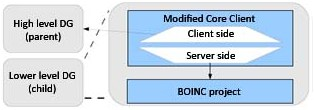
\includegraphics[height=30mm]{SZTAKI_LDG.jpg}
  \caption{Hierarchy client \cite{balaton}}
\end{center}
\end{figure}

\paragraph{}
Hierarchical mode is implemented by a hierarchy client, which is run on the child LDG server. This way, the parent does not have to be aware of the hierarchy; it sees the child as one powerful client. The hierarchy client has two sides (see Figure 1): a master side which puts retrieved work-units in the database of the LDG and gets the computed results, and a client side which retrieves work-units from the parent and uploads results \cite{balaton}.

\subsection{Load Balancing}

\paragraph{}
A size-$n$ problem is embarrassingly parallel if it is composed of $n$ independent tasks, which when solved in parallel, the computation process achieves a speed-up of O($n$) with very little interprocess communication. One example of this is a loop with $n$ independent iterations. The $i$th loop iterate is independent if it doesn't require the result of the computation of the $(i-1)$th iterate, and it does not affect the other iterates \cite{pabico}.

\paragraph{}
To ensure efficiency of embarrassingly parallel applications, various loop scheduling algorithms have been designed and evaluated by several researchers. These algorithms find an efficient policy to effectively distribute the tasks to the processors such that few, if not none, will be idle. There are two types of scheduling algorithms: the static or offline scheduling and the dynamic or online scheduling.

\paragraph{}
In static scheduling, the decision of which processor will work on a task is done before program execution by the programmer. The most trivial static scheduling decision for a given problem with n number of tasks on a computational infrastructure with p number of processors, where $p<<n$, is to assign $n/p$ tasks to each processor. With this scheduling decision, performance degradation of the parallel system will happen if the actual distribution of the task execution times is skewed. And since the assignment happened at compile time, the idle processors cannot help in computing the load of the busy ones, increasing the realized execution time and effectively reducing speed-up \cite{pabico}.

\paragraph{}
For this reason, using the static scheduling, also referred to as deterministic scheduling, is only advisable when all information about tasks to be scheduled (i.e. execution times) and their relation to one another is entirely known prior to execution time. These information will be used to make a decision as to how each task is to have a static assignment of which particular processor it is assigned to when it is submitted for execution \cite{el-rewini}.

\paragraph{}
Dynamic scheduling algorithms, on the other hand, make the decision of which processor will perform a task on the fly as the program executes. These algorithms are fixed-size chunking (FSC), guided self scheduling (GSS), factoring (FACT), weighted factoring (WFACT), adaptive weighted factoring (AWF), and adaptive factoring (AF).

\paragraph{}
In FSC, the tasks are grouped into chunks of size $c$, usually chosen to be $c<<n/p$ and, as much as possible, is divisible by p (i.e. $p$ modulo $c$ is 0). The first $p$ chunks of tasks are initially distributed by the scheduler\footnote{In practice, the scheduler is usually $P_0$.} to the processors\footnote{If $P_0$ is the scheduler, it also distributes to itself.}. When a processor happens to be assigned with tasks that have short execution times, the processor will finish early. And since there are still tasks to be computed, it can request the scheduler for the next chunk of tasks, incurring a cost $tc$ brought about by communication latency. The communication latency is incurred by both the scheduler and the requesting processors, and happens when the processor requests for the next chunk until the scheduler answers with the next assignment. For scientific applications with independent loops, only the indexes of the iterates are communicated by the scheduler, incurring a smaller $tc$. At the end of the computation, the processors’ finishing times will vary at a maximum of $c$, improving the realized execution time of the scientific application.

\paragraph{}
The GSS scheduling is simply implemented as FSC with $c=1$. The communication latency is incurred by both the scheduler and the requesting processors, and happens when the processor requests for the next chunk until the scheduler answers with the next assignment. For scientific applications with independent loops, only the indexes of the iterates are communicated by the scheduler, incurring a smaller $tc$. At the end of the computation, the processors’ finishing times will also vary at a maximum of $c$, improving the realized execution time of the scientific application.

\paragraph{}
FACT is a scheduling algorithm that implements a variable sized chunk $c$ using some factoring rules. The idea of this scheme is to accommodate load imbalances caused by predictable phenomena, such as data-access latency due to I/O bursts and OS interference. One example of a factoring rule is to schedule chunks of tasks such that $c$ is a fixed factor of those remaining. For example, setting the factor to be $0 < \gamma < 1$, then $P_0$ is assigned $\gamma\times n$ tasks and $P_1$ is assigned $\gamma^2\times n$ tasks. In general, $P_j$ is assigned $\gamma^{j+1}  n$ tasks. The selection of $c$ requires that the chunks have high probability of being completed by the processors before the optimal time. The chunk sizes are dynamically computed by the scheduler at runtime. When computing for the larger chunks, the processors incur a relatively low communication overhead. The unevenness of the respective finishing times of the larger chunks can be smoothed over by the smaller chunks made available towards the end of the computation.

\paragraph{}
WFACT was proposed to take into consideration the effect of processor heterogeneity of the underlying runtime system. This method, derived from FACT, computes c by taking into consideration the relative computing speed of the processor as a weight for γ during the time of computation. At the start of the computation, the relative processing speeds of the processors will be profiled resulting in an array $S = \{s_0, s_1,\dots, s_{p−1}\}$ of relative processor speeds corresponding to processors $P_0, P_1, \dots, P_{p−1}$. A vector of chunk sizes $C = \{c_0, c_i,\dots, c_{p−1}\}$ will be computed from $c_i = si/smax \times\gamma$, where $smax = max(s_0, s_1,\dots, s_{p−1})$. These chunk sizes are statically assigned to processors and are considered to remain unchanged throughout the entire lifespan of the application. Experiments involving network of workstations, where relative processor speeds are extremely heterogeneous, have shown that WFACT significantly outperformed FACT.

\paragraph{}
In computational environments where processor workloads vary during the computation, chunk sizes must be assigned to processors dynamically. Many applications whose solutions require a number of iterations over the computation space are expected to benefit from a dynamic adjustment of weights after finishing each chunk of tasks. This aspect is addressed by the AWF, wherein the relative processor speeds are profiled after every computation of a chunk.

\paragraph{}
AFACT was developed as a general model for FACT, WFACT, and AWF schemes. AFACT’s flexibility is suited for highly irregular applications, where even within an iteration over the computation space, the load becomes unpredictably imbalanced. Because of its generality, AFACT reduces into FACT, WFACT, or AWF under specific conditions of processor speeds and task workloads \cite{pabico}.

\subsection{Loop Scheduling on Desktop Grids}

\paragraph{}
A study shows that the loop scheduling algorithms are effective in balancing the load of embarrassingly parallel applications \cite{pabico}.

\paragraph{}
However, the loop scheduling algorithms\rq\ performances on DGs have not yet been presented and analyzed as of now.

\section{Objectives}

\paragraph{}
The main objective of this study is to implement the Loop Scheduling algorithms to show which of them are best for developing or optimizing embarrassingly parallel applications for DGs on four different scenarios with varying distribution of task execution times. The Synthetic Embarrassingly Parallel Application (SEPA), which is a trivial embarrassingly parallel problem, is used as test bed for the implementations.

\paragraph{}
Specifically, the following are done in this study:

\begin{itemize}
	\item{Design and implement the SEPA}
	\item{Implement the loop scheduling algorithms using the SEPA as test bed over DG systems}
	\item{Compare the performance of each scheduling algorithm over an increasing number of processors in varying SEPA modes}
\end{itemize}

\section{Methodology}

\subsection{Synthetic Embarrassingly Parallel Application}

\paragraph{}
The SEPA is a program designed to have four modes---each having different distribution of task execution times. These four modes are: \textsf{EQUAL}, \textsf{FRONT-HEAVY}, \textsf{TAIL-HEAVY}, and \textsf{RANDOM}.

\paragraph{}
In \textsf{EQUAL} mode, each of the tasks $T_i, \forall i=0,1,\dots,n$ has an identical execution time $x$. This mode was used to simulate embarrassingly parallel applications where each of the independent iterations have identical load.

\textsf{\\pseudo-code:}
\begin{verbatim}
1    x = any integer;
2    for(i=0 to n-1){
3         fibonacci(x);
4    }
\end{verbatim}

\paragraph{}
In \textsf{FRONT-HEAVY} mode, the beginning of the loop has a relatively large execution time $x$ that decreases for iterations $T_i$ as $i$ approaches $n$. In this mode, the distribution of task execution times is skewed to the left. This mode was used to simulate embarrassingly parallel applications where the load is relatively heavy in the start of the program but gradually lightens as it ends. 

\textsf{\\pseudo-code:}
\begin{verbatim}
1    x = large integer;
2    for(i=0 to n-1){
3        fibonacci(x=decrease(x));
4    }
\end{verbatim}

\paragraph{}
The \textsf{TAIL-HEAVY} mode is the opposite of \textsf{FRONT-HEAVY}. The beginning of the loop has a relatively small execution time $x$ that gradually increases for iterations $T_i$ as $i$ approaches $n$. In this mode, the distribution of the task execution times is skewed to the right. This mode was used to simulate embarrassingly parallel applications where the load is relatively light in the start of the program but gradually weighs up as it ends.

\textsf{\\pseudo-code:}
\begin{verbatim}
1    x = small integer;
2    for(i=0 to n-1){
3         fibonacci(x=increase(x));
4    }
\end{verbatim}

\paragraph{}
In the \textsf{RANDOM} mode, the execution times of the iterations does not have any pattern. This mode was used to observe which of the loop scheduling algorithms is best when dealing with embarassingly parallel applications with independent iterations that has unpredictable load sizes.

\textsf{\\pseudo-code:}
\begin{verbatim}
1   for(i=0 to n-1){
2        fibonacci(x=random());
3   }
\end{verbatim}

\subsection{Implementation of Loop Scheduling Algorithms}

\paragraph{}
Each of the loop scheduling algorithms---one static scheduling (\textsf{STATIC}) and four dynamic scheduling (\textsf{FSC}, \textsf{GSS}, \textsf{FACT}, \textsf{WFACT})---was implemented as Master-Worker programs where the Master computers distribute the tasks to the Workers. Each program was installed in the ten DGs with varying sizes (2, 4, 6, ... upto 20 computers). In the implementations, the Master computer distributed the tasks to all the computers by sending the lower and upper bounds of the portion of the loop that needs to be computed in the SEPA. The Workers, on the other hand, received the bounds and ran the SEPA. After processing the assigned portion of the loop, the Workers sent the results to the Master PC and requested for another set of tasks. The Master PC, in response, sent the next portion of the loop that needs processing. This request-response cycles between the Master computers and the Workers went on until all the loops were processed.

\paragraph{}
AF and AWF are not included in the implementations in this study because they are just generalizations of FACT, WFACT. 

\paragraph{}
The following are the pseudo-codes for the different scheduling algorithms:\\\\
p\textsf{ = number of PCs}\\
n\textsf{ = number of loop iterations}\\
c\textsf{ = chunk size}

\paragraph{\textsf{STATIC}}
\begin{verbatim}
1    c = n/p;
2    for(i=0 to p-1){
3         send chunk[i] to processor P[i]
4            lowerbound l = i*c
5            and
6            upperbound u = ((i+1)*c)-1
7    }
\end{verbatim}

\paragraph{\textsf{FSC}}
\begin{verbatim}
 1    c = any integer such that
 2        c << n/p, and if possible
 3        p modulo c = 0;
 4
 5    /*send first p chunks to all PCs*/
 6    for(i=0 to p-1){
 7         send chunk[i] to processor P[i]
 8            lowerbound l = i*c
 9            and
10           upperbound u = ((i+1)*c)-1
11    }
12
13    until all tasks are done:
14        respond to a requesting processor p
15        send next chunk of tasks
\end{verbatim}


\paragraph{\textsf{GSS}}
This will be the same as FSC except that the chunk size $c$ will be set to 1.\\

\paragraph{\textsf{FACT}}
\begin{verbatim}
 1    /*c is a fixed factor of remaining
 2      tasks*/
 3    f = any number such that 0 < f < 1;
 4
 5    /*send first p chunks to all PCs*/
 6    for(i=0 to p-1){
 7         c = (f^i*n);
 8         send chunk[i] to processor P[i]
 9            lowerbound l = i*c
10           and
11           upperbound u = ((i+1)*c)-1
12    }
13
14    do until all tasks are done:
15    respond to a requesting processor p
16         compute c
17         send next chunk of tasks
\end{verbatim}

\paragraph{\textsf{WFACT}}
\begin{verbatim}
 1    /*c is a fixed factor of remaining
 2        tasks*/
 3    /*f[i] is the the relative speeds
 4        of processor P[i]*/
 5
 6    /*initally all of the relative speeds
 7        of all the processors are equal*/
 8    for(i=0 to p-1){
 9         f[i] = any number
10                 such that 0<f[i]<1;
11    } 
12    /*send first p chunks to all PCs*/
13    for(i=0 to p-1){
14        c = (f[i]*n);
15        /*update f[i]*/
16        f[i] = relative speed of P[i];
17         send chunk[i] to processor P[i]
18            lowerbound l = i*c
19            and
20            upperbound u = ((i+1)*c)-1
21    }
22
23    do until all tasks are done:
24    respond to a requesting processor p
25         compute c
26         send next chunk of tasks
\end{verbatim}

\subsection{Comparison of Performances}

\paragraph{}
After four replications of the implementations, several performance metrics were recorded and then compared with each other. Since the Master computers were the ones which sent tasks and waited for the requests from the Workers until the end, they were the ones that started first and terminated last in every implementation. Therefore, the execution times of the progams in the Master computers were the system parallel time $\tau_p$ which is the sum total of the time spent for computation $t_{comp}$ and the time spent for communication and waiting $t_c$. Also, the parallel cost $C_p$ was computed by multiplying the parallel time $\tau_p$ by the number of processors $p$ in the DG\cite{pabico}. The parallel cost $C_p$ is used to measure the overall performance of a parallel computing system.

\section{Results and Discussions}

\paragraph{}
The implementations of the loop scheduling algorithms on the DGs using SEPA as a test bed on four modes (\textsf{EQUAL}, \textsf{FRONT-HEAVY}, \textsf{TAIL-HEAVY}, and \textsf{RANDOM}) shows that the scheduling algorithms effectively balances the work load to the DGs and reduces the execution times relative to when SEPA is executed sequentially in a single PC.

\paragraph{}
Figures 2, 3, 4, and 5 are comparisons of the execution times of each of the implementations. hahahaha :)

\begin{figure}[h]
\begin{center}  
  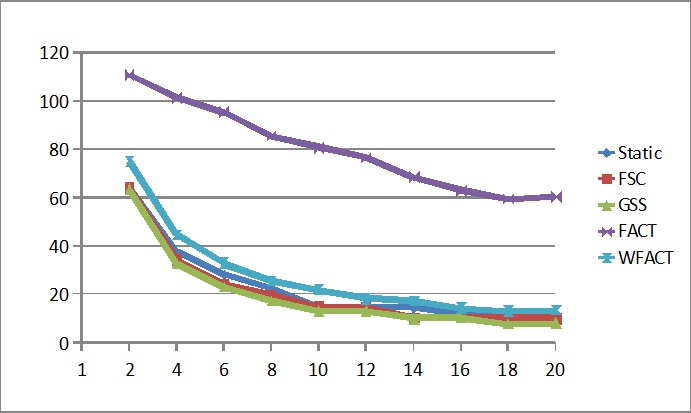
\includegraphics[height=45mm]{graphs/equal.jpg}
  \caption{SEPA on \textsf{EQUAL} mode}
\end{center}
\end{figure}

\begin{figure}[h]
\begin{center}  
  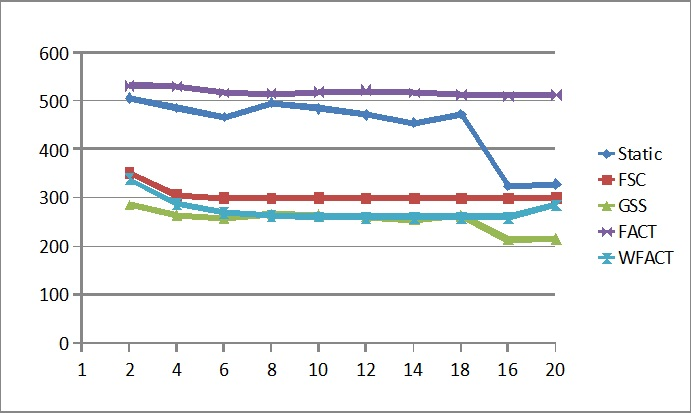
\includegraphics[height=45mm]{graphs/front.jpg}
  \caption{SEPA on \textsf{FRONT-HEAVY} mode}
\end{center}
\end{figure}

\begin{figure}[h]
\begin{center}  
  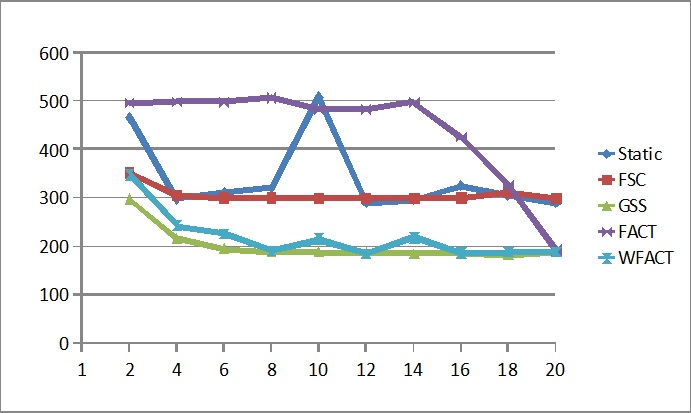
\includegraphics[height=45mm]{graphs/tail.jpg}
  \caption{SEPA on \textsf{TAIL-HEAVY} mode}
\end{center}
\end{figure}

\begin{figure}[h]
\begin{center}  
  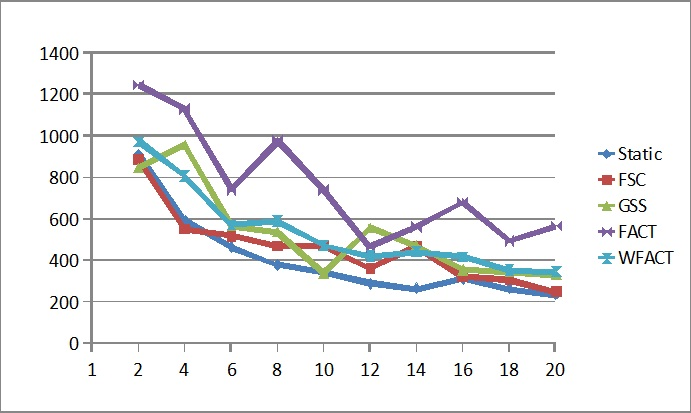
\includegraphics[height=45mm]{graphs/random.jpg}
  \caption{SEPA on \textsf{RANDOM} mode}
\end{center}
\end{figure}

\paragraph{}

\begin{thebibliography}{8}
	\bibitem{balaton}
\begin{flushleft}Z. Balaton, G. Gomb\'as, P. Kacsuk, \'A. Kornafeld, J. Kovács, A.C. Marosi, G. Vida, N. Podhorszki, and T. Kiss. \emph{SZTAKI Desktop Grid: a Modular and Scalable Way of Building Large Computing Grids}. IEEE, 2007.
\end{flushleft}

	\bibitem{codenotti}
\begin{flushleft}B. Codenotti and M. Leoncini.\emph{Introduction to Parallel Processing}. Addison-Wesley Publishing Inc., 1993.
\end{flushleft}

	\bibitem{el-rewini}
\begin{flushleft}H. El-Rewini, T.G. Lewis, and H.H. Ali. \emph{Task  Scheduling in Parallel and Distributed Systems}. Prentice-Hall Inc., 1994.
\end{flushleft}

	\bibitem{marosi}
\begin{flushleft}A.C. Marosi, G. Gomb´as, and Z. Balaton. \emph{Secure application deployment in the hierarchical local desktop grid}. In Proceedings of DAPSYS 2006 6th Austrian-Hungarian Workshop on Distributed and Parallel Systems, Innsbruck, Austria, 2006.
\end{flushleft}

	\bibitem{morse}
\begin{flushleft}H.S. Morse. \emph{Practical Parallel Computing}. Academic Press, Inc., 1994.
\end{flushleft}

	\bibitem{pabico}
\begin{flushleft}J.P. Pabico. \emph{Dynamic Load Balancing Algorithms for Embarrassingly Parallel Tasks}. Computing Society of the Philippines, 2009.
\end{flushleft}

	\bibitem{desktopgrid.hu}
\begin{flushleft}Computer Automation Research Institute (SZTAKI) of the Hungarian Academy of Sciences (MTA), (2006). Available: http://www.desktopgrid.hu
\end{flushleft}

	\bibitem{tabirca}
\begin{flushleft}T. Tabirca, S. Tabirca, and L.T. Yang. \emph{An O(log(p)) Algorithm for the Discrete Feedback Guided Dynamic Loop Scheduling}. In Proceedings of the 20th International Conference on Advanced Information Networking and Applications (AINA’06), 2006.
\end{flushleft}

\end{thebibliography}
\end{document}
